\chapter{Applying Computer Software in Calculating Machine Elements}

\section{Aim}
Helping students understand the method, how to use the design software to select and test the general machine elements.
\section{Technical rules on safety}
Students must comply with the technical rules on safety in the laboratory.
\section{Experimental report}
\subsection{Problem}
Given the transmission system as shown in below figure.
\begin{figure}
	\centering
	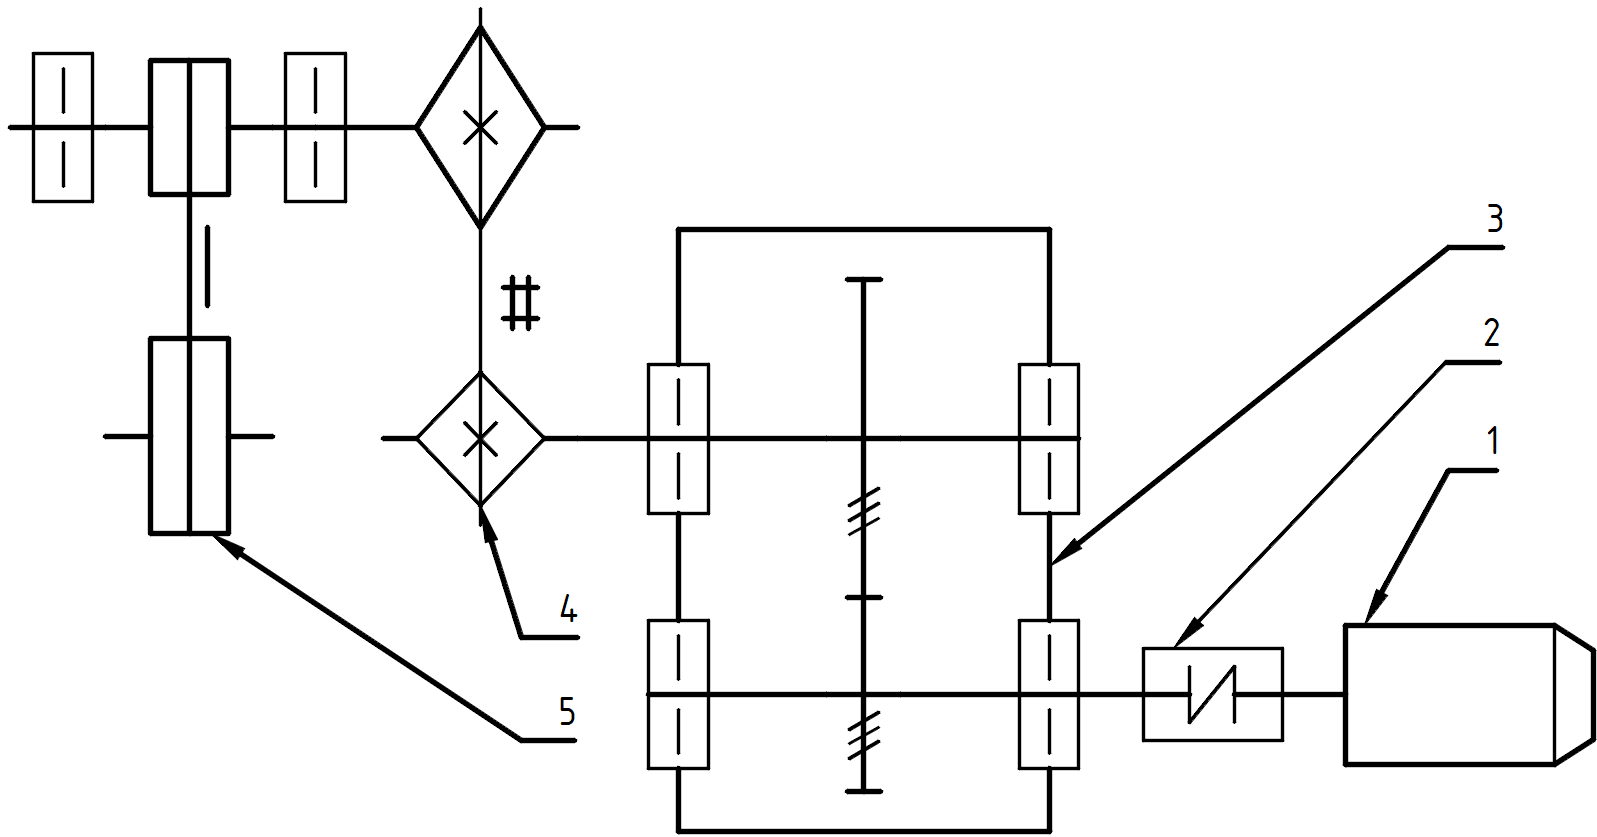
\includegraphics[width=150mm]{system.png}
	\caption{Transmission system for the blender}
	\label{blender}
\end{figure}

%\begin{table}
%	content
%\end{table}
\subsubsection{Initial data}
\begin{itemize}
	\item Capacity of blender: $ P_3 = 4\unit{(kW)} $
	\item Number of revolution of blender:  $ n_3 \unit{(rpm)} $
	\item Service life cycle: $ L_h = 8\unit{(years)} $
	\item 1-way rotation, work 2 shifts, static load (300 working days per year, 8 hours per 1 working shift)
	\item Number of revolution of motor: $ n_{dc} =1420 \unit{(rpm)}$.
	\item Efficiency:
	\begin{itemize}
		\item Belt drive $ \eta_d = 0.95 $.
		\item Spur gear drive $ \eta_{br} = 0.96 $.
		\item Bearings $ \eta_{ol} = 0.99 $.
		\item Chain drive $ \eta_x = 0.95 $.
	\end{itemize}
\item The gears are calculated by ISO standard, the material is ENC60, the coefficients including $ K_A = 1 $, $ K_{Hv} = 1.2 $, $ K_{H\beta} = 1.2 $, $ K_{H\alpha} = 1 $ are input into Autodesk Inventor.
\item The belt drive is calculated by DIN 2215 standard. Choose $ d_1 = 180\unit{(mm)} $, center distance $ a = d_2 $, the belt length, DIN belt type. The coefficient such as $ P_{RB} = 3.8\unit{(kW)} $, $ k_1 = 1.2 $.
\item The chain is selected by ISO 606:2004 (EU) standard.
\end{itemize}
\begin{center}
	\begin{longtable}{C{0.6cm}rrrrC{0.6cm}rrrrC{0.6cm}rrrr}
		\toprule
		\multirow{2}{*}{Pr} & \multicolumn{4}{c}{Parameters} & \multirow{2}{*}{Pr} & \multicolumn{4}{c}{Parameters} & \multirow{2}{*}{Pr} & \multicolumn{4}{c}{Parameters}\\
		\cmidrule{2-5}\cmidrule{7-10}\cmidrule{12-15} & $ P_3 $ & $ u_1 $ & $ u_2 $ & $ u_3 $ & & $ P_3 $ & $ u_1 $ & $ u_2 $ & $ u_3 $ & & $ P_3 $ & $ u_1 $ & $ u_2 $ & $ u_3 $\\\midrule
		\endfirsthead
		& $ P_3 $ & $ u_1 $ & $ u_2 $ & $ u_3 $ & & $ P_3 $ & $ u_1 $ & $ u_2 $ & $ u_3 $ & & $ P_3 $ & $ u_1 $ & $ u_2 $ & $ u_3 $\\\midrule\endhead
		\bottomrule\endfoot
		\bottomrule\caption{Projects}\endlastfoot
		\rowcolor{lightgray!20}{\cellcolor[HTML]{C0C0C0}}1 &2.5&2&2 & 3 &{\cellcolor[HTML]{C0C0C0}}31 & 6.5&4&2&3  &{\cellcolor[HTML]{C0C0C0}}61&12&3&2&4\\
		{\cellcolor[HTML]{C0C0C0}}2 &2.5&2&2.24&4&{\cellcolor[HTML]{C0C0C0}}32&7&3&2.24&3   &{\cellcolor[HTML]{C0C0C0}}62&12&4&2.24&2\\
		\rowcolor{lightgray!20}{\cellcolor[HTML]{C0C0C0}}3 &2.5&4&2.5&4 &{\cellcolor[HTML]{C0C0C0}}33&7&4&2.5&4    &{\cellcolor[HTML]{C0C0C0}}63&12.5&3&2.5&3\\
		{\cellcolor[HTML]{C0C0C0}}4 &3&2&3.15&3  &{\cellcolor[HTML]{C0C0C0}}34&7&3&3.15&4&   {\cellcolor[HTML]{C0C0C0}}64&12.5&3&3.15&4\\
		\rowcolor{lightgray!20}{\cellcolor[HTML]{C0C0C0}}5 &3&2&3.55&3  &{\cellcolor[HTML]{C0C0C0}}35&7&2&3.55&3&   {\cellcolor[HTML]{C0C0C0}}65&12.5&4&3.55&2\\
		{\cellcolor[HTML]{C0C0C0}}6 &3&4&4&2     &{\cellcolor[HTML]{C0C0C0}}36&7&3&4&4&      {\cellcolor[HTML]{C0C0C0}}66&12.5&3&4&4\\
		\rowcolor{lightgray!20}{\cellcolor[HTML]{C0C0C0}}7 &3&2&2&3     &{\cellcolor[HTML]{C0C0C0}}37&7.5&4&2&2&    {\cellcolor[HTML]{C0C0C0}}67&12.5&4&2&3\\
		{\cellcolor[HTML]{C0C0C0}}8 &3&4&2.24&3  &{\cellcolor[HTML]{C0C0C0}}38&7.5&4&2.24&3& {\cellcolor[HTML]{C0C0C0}}68&12.5&4&2.24&2\\
		\rowcolor{lightgray!20}{\cellcolor[HTML]{C0C0C0}}9&3.5&3&2.5&2  &{\cellcolor[HTML]{C0C0C0}}39&7.5&4&2.5&3&  {\cellcolor[HTML]{C0C0C0}}69&13&4&2.5&4\\
		{\cellcolor[HTML]{C0C0C0}}10&3.5&4&3.15&2&{\cellcolor[HTML]{C0C0C0}}40&8&4&3.15&3&   {\cellcolor[HTML]{C0C0C0}}70&13&3&3.15&4\\
		\rowcolor{lightgray!20}{\cellcolor[HTML]{C0C0C0}}11&3.5&3&3.55&2&{\cellcolor[HTML]{C0C0C0}}41&8&4&3.55&2&   {\cellcolor[HTML]{C0C0C0}}71&13&2&3.55&2\\
		{\cellcolor[HTML]{C0C0C0}}12&3.5&3&4&4   &{\cellcolor[HTML]{C0C0C0}}42&8&4&4&3&      {\cellcolor[HTML]{C0C0C0}}72&13&3&4&2\\ 
		\rowcolor{lightgray!20}{\cellcolor[HTML]{C0C0C0}}13&4&4&2&3&     {\cellcolor[HTML]{C0C0C0}}43&8&2&2&3&      {\cellcolor[HTML]{C0C0C0}}73&13&4&2&3\\
		{\cellcolor[HTML]{C0C0C0}}14&4&3&2.24&3  &{\cellcolor[HTML]{C0C0C0}}44&8.5&2&2.24&2& {\cellcolor[HTML]{C0C0C0}}74&13&3&2.24&3\\
		\rowcolor{lightgray!20}{\cellcolor[HTML]{C0C0C0}}15&4&3&2.5&4&   {\cellcolor[HTML]{C0C0C0}}45&8.5&2&2.5&3&  {\cellcolor[HTML]{C0C0C0}}75&13&2&2.5&4\\
		{\cellcolor[HTML]{C0C0C0}}16&4&4&3.15&2  &{\cellcolor[HTML]{C0C0C0}}46&8.5&3&3.15&2& {\cellcolor[HTML]{C0C0C0}}76&13&4&3.15&4\\
		\rowcolor{lightgray!20}{\cellcolor[HTML]{C0C0C0}}17&4&3&3.55&3&  {\cellcolor[HTML]{C0C0C0}}47&8.5&2&3.55&2& {\cellcolor[HTML]{C0C0C0}}77&13.5&4&3.55&4\\
		{\cellcolor[HTML]{C0C0C0}}18&4&3&4&2&     {\cellcolor[HTML]{C0C0C0}}48&8.5&4&4&3&    {\cellcolor[HTML]{C0C0C0}}78&14&3&4&2\\
		\rowcolor{lightgray!20}{\cellcolor[HTML]{C0C0C0}}19&4&4&2&3&     {\cellcolor[HTML]{C0C0C0}}49&9.5&2&2&3&    {\cellcolor[HTML]{C0C0C0}}79&14&2&2&4\\
		{\cellcolor[HTML]{C0C0C0}}20&4&4&2.24&3&  {\cellcolor[HTML]{C0C0C0}}50&9.5&4&2.24&4& {\cellcolor[HTML]{C0C0C0}}80&14&3&2.24&2\\
		\rowcolor{lightgray!20}{\cellcolor[HTML]{C0C0C0}}21&4.5&3&2.5&2& {\cellcolor[HTML]{C0C0C0}}51&10&4&2.5&4&   {\cellcolor[HTML]{C0C0C0}}81&14&3&2.5&4\\
		{\cellcolor[HTML]{C0C0C0}}22&4.5&3&3.15&3&{\cellcolor[HTML]{C0C0C0}}52&10&4&3.15&3&  {\cellcolor[HTML]{C0C0C0}}82&14.5&4&3.15&4\\
		\rowcolor{lightgray!20}{\cellcolor[HTML]{C0C0C0}}23&5.5&4&3.55&4&{\cellcolor[HTML]{C0C0C0}}53&10.5&4&3.55&4&{\cellcolor[HTML]{C0C0C0}}83&14.5&3&3.55&4\\
		{\cellcolor[HTML]{C0C0C0}}24&5.5&2&4&3&   {\cellcolor[HTML]{C0C0C0}}54&10.5&2&4&4&   {\cellcolor[HTML]{C0C0C0}}84&15&3&4&2\\
		\rowcolor{lightgray!20}{\cellcolor[HTML]{C0C0C0}}25&6&3&2&4&     {\cellcolor[HTML]{C0C0C0}}55&10.5&2&2&4&   {\cellcolor[HTML]{C0C0C0}}85&15&2&2&3\\
		{\cellcolor[HTML]{C0C0C0}}26&6&2&2.24&4&  {\cellcolor[HTML]{C0C0C0}}56&10.5&2&2.24&2&{\cellcolor[HTML]{C0C0C0}}86&15&4&2.24&3\\
		\rowcolor{lightgray!20}{\cellcolor[HTML]{C0C0C0}}27&6&4&2.5&4&   {\cellcolor[HTML]{C0C0C0}}57&10.5&2&2.5&2& {\cellcolor[HTML]{C0C0C0}}87&15.5&3&2.5&3\\
		{\cellcolor[HTML]{C0C0C0}}28&6&4&3.15&3&  {\cellcolor[HTML]{C0C0C0}}58&11&4&3.15&3&  {\cellcolor[HTML]{C0C0C0}}88&15.5&3&3.15&4\\
		\rowcolor{lightgray!20}{\cellcolor[HTML]{C0C0C0}}29&6&4&3.55&3&  {\cellcolor[HTML]{C0C0C0}}59&11&3&3.55&3&  {\cellcolor[HTML]{C0C0C0}}89&16&4&3.55&2\\
		{\cellcolor[HTML]{C0C0C0}}30&6.5&2&4&3&   {\cellcolor[HTML]{C0C0C0}}60&11.5&2&4&4&   {\cellcolor[HTML]{C0C0C0}}90&16&4&4&3\\
		\label{project}
	\end{longtable}
\end{center}

\subsection{Results}
\subsubsection{The distribution table of transmission ratio}
\begin{center}
	\rowcolors{3}{}{lightgray!20}
	\begin{longtable}{lrrrr}
		\toprule
		\multirow{2}{*}{Parameters} & \multicolumn{4}{c}{Shaft}\\
		\cmidrule{2-5}  &Motor & I & II & III\\\midrule\endfirsthead
		\bottomrule\caption{Table of transmission ratio}\endlastfoot
		$ P\unit{(kW)} $ & 4.758 & 4.475 & 4.253 & 4\\
		$ u $ & $ 1\rightarrow1 $ & $ 1\rightarrow3 $ & $ 3\rightarrow2.5 $ & $ 2.5\rightarrow4 $\\
		$ n\unit{(rpm)} $ & 1420 & 473.33 & 189.33 & 47.33 \\
		$ T\unit{(N\cdot mm)} $ & 31999 & 90288 & 214526 & 807099
	\end{longtable}
\end{center}

\subsubsection{Table of gear drive parameters}
\begin{center}
	\rowcolors{1}{}{lightgray!20}
	\begin{longtable}{clr}
		\toprule
		No. & \multicolumn{1}{c}{Parameter} & \multicolumn{1}{c}{Result}\\
		\midrule\endfirsthead
		\toprule
		No. & \multicolumn{1}{c}{Parameter} & \multicolumn{1}{c}{Result}\\
		\midrule\endhead
		\bottomrule\endfoot
		\bottomrule
		\caption{Design specifications of the gear drive}
		\endlastfoot
		1 & Selected material & EN C60\\
		2 & Center distance & $ a=160\unit{(mm)} $\\
		3 & Module & $ m=4\unit{(mm)} $\\
		4 & Number of teeth & $ z_1 =23 $\\
		5 & Number of teeth & $ z_2 =57 $\\
		6 & Pitch circle diameter & $ d_1=92\unit{(mm)} $\\
		7 & Pitch circle diameter & $ d_2=228\unit{(mm)} $\\
		8 & Face width & $ b_1=64\unit{(mm)} $\\
		9 & Face width & $ b_2=60\unit{(mm)} $\\
		10 & Radial force & $ F_r=714.346\unit{(N)} $\\
		11 & Tangential force & $ F_t=1962.649\unit{(N)} $\\
		12 & Gear speed & $ v=2.28\unit{(m/s)} $
	\end{longtable}
\end{center}
\begin{figure}
	\centering
	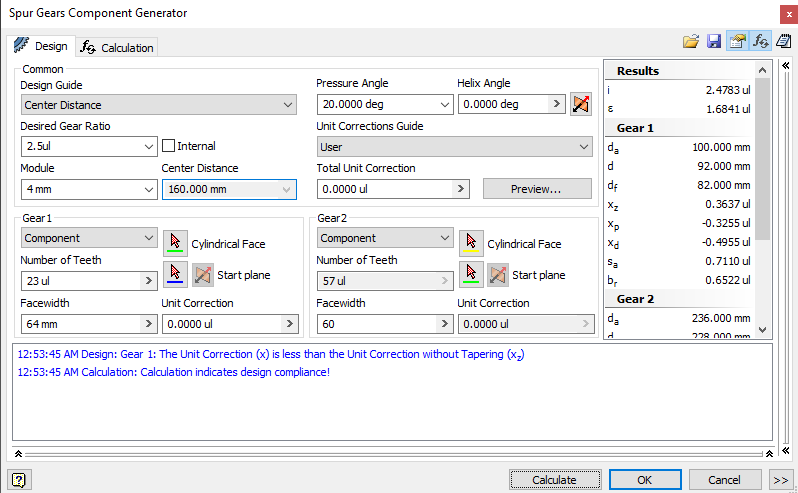
\includegraphics[width=150mm]{geardesign.png}
	\caption{Gear design tab}
	\label{geardesign}
\end{figure}
\begin{figure}
	\centering
	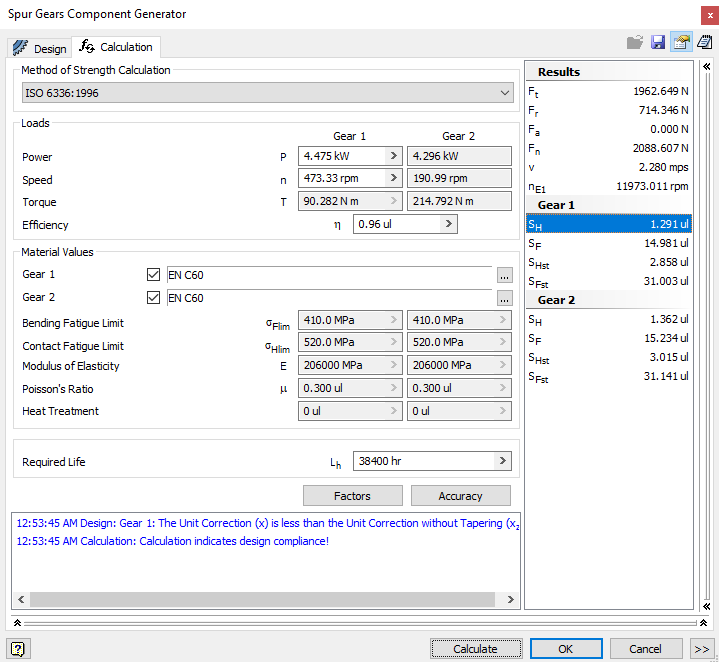
\includegraphics[width=150mm]{gearcalculation.png}
	\caption{Gear calculation tab}
	\label{gearcalculation}
\end{figure}
\begin{figure}
	\centering
	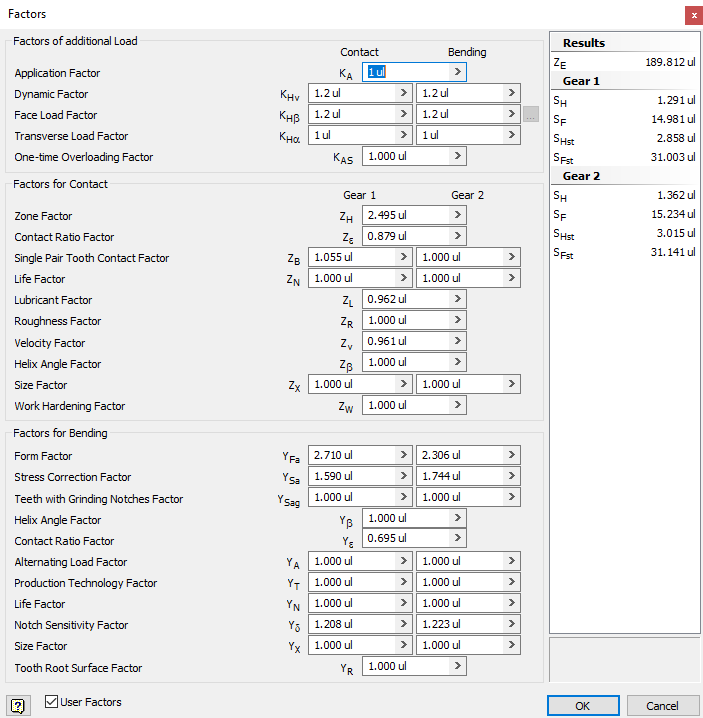
\includegraphics[width=150mm]{gearfactor.png}
	\caption{Gear factors tab}
	\label{gearfactor}
\end{figure}
\begin{figure}
	\centering
	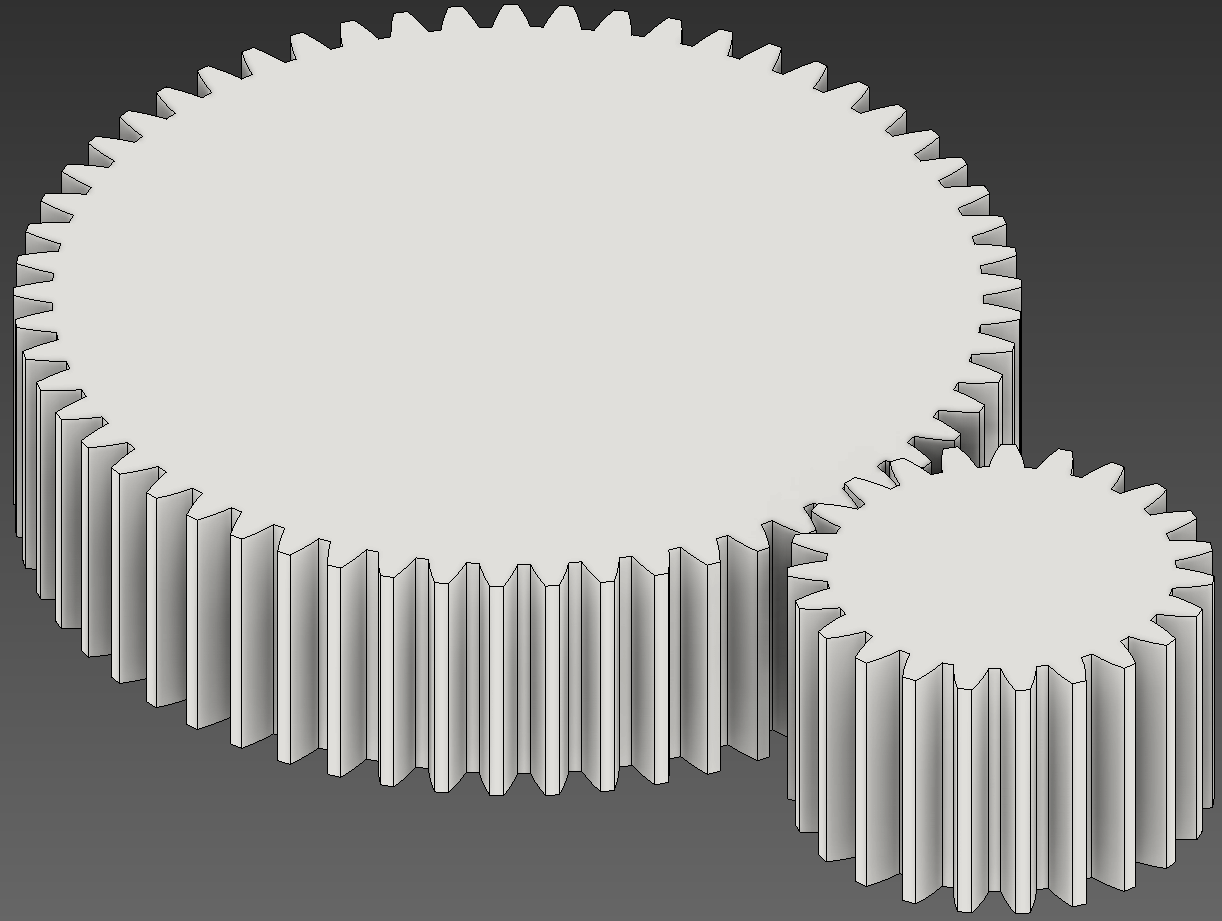
\includegraphics[width=150mm]{gear.png}
	\caption{Gear drive model}
	\label{gear}
\end{figure}

\subsubsection{The belt drive parameters table}
\begin{center}
	\rowcolors{1}{}{lightgray!20}
	\begin{longtable}{clr}
		\toprule
		No. & \multicolumn{1}{c}{Parameter} & \multicolumn{1}{c}{Result}\\
		\midrule\endfirsthead
		\toprule
		No. & \multicolumn{1}{c}{Parameter} & \multicolumn{1}{c}{Result}\\
		\midrule\endhead
		\bottomrule\endfoot
		\bottomrule
		\caption{Design specifications of the belt drive}
		\endlastfoot
		1 & Belt type & V-Belt DIN 2215 (17x2240)\\
		2 & Number of belt & $ z=3 $\\
		3 & Belt speed & $ v=13.383\unit{(m/s)} $\\
		4 & Initial tensile force & $ F_v=700.197\unit{(N)} $\\
		5 & Tensile force on each side & $ F_t=125.165\unit{(N)} $\\
		6 & Tensile force on the tight side & $ F_1=553.254\unit{(N)} $\\
		7 & Tensile force on the slack side & $ F_2=197.734\unit{(N)} $\\
		8 & Tangential force & $ F_p=355.521\unit{(N)} $\\
		9 & Radial force  & $ F_r =711.895\unit{(N)}$\\
		10 & Wrap angle & $ \alpha_1 = 137.61^\circ, \alpha_2= 222.39^\circ $\\
		11 & Belt length & $ L_d=2283\unit{(mm)} $\\
		12 & Pulley width & $ B=63\unit{(mm)} $\\
		13 & Center distance & $ C=572.572\unit{(mm)} $\\
	\end{longtable}
\end{center}
\begin{figure}
	\centering
	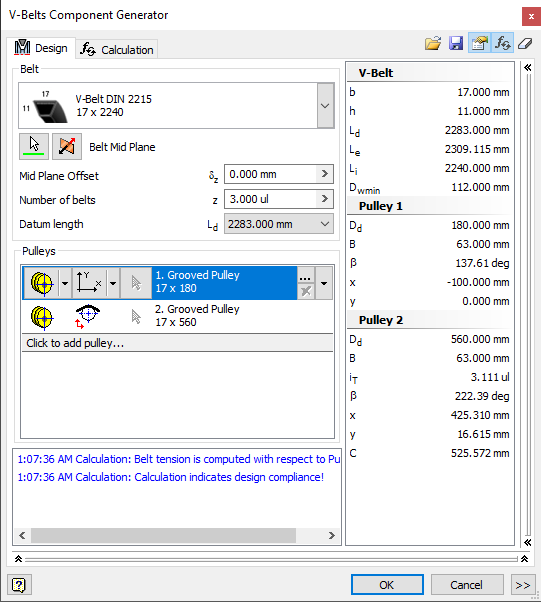
\includegraphics[width=150mm]{beltdesign.png}
	\caption{Belt design tab}
	\label{beltdesign}
\end{figure}
\begin{figure}
	\centering
	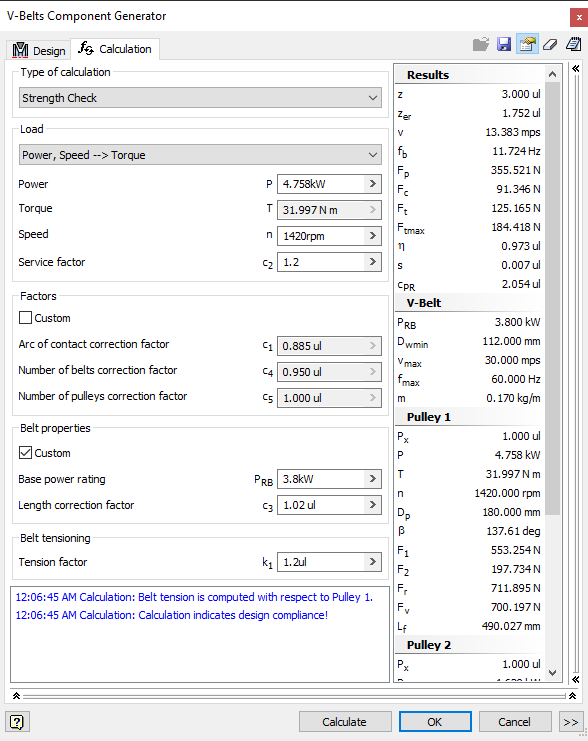
\includegraphics[width=150mm]{beltcalculation.png}
	\caption{Belt calculation tab}
	\label{beltcalculation}
\end{figure}
\begin{figure}
	\centering
	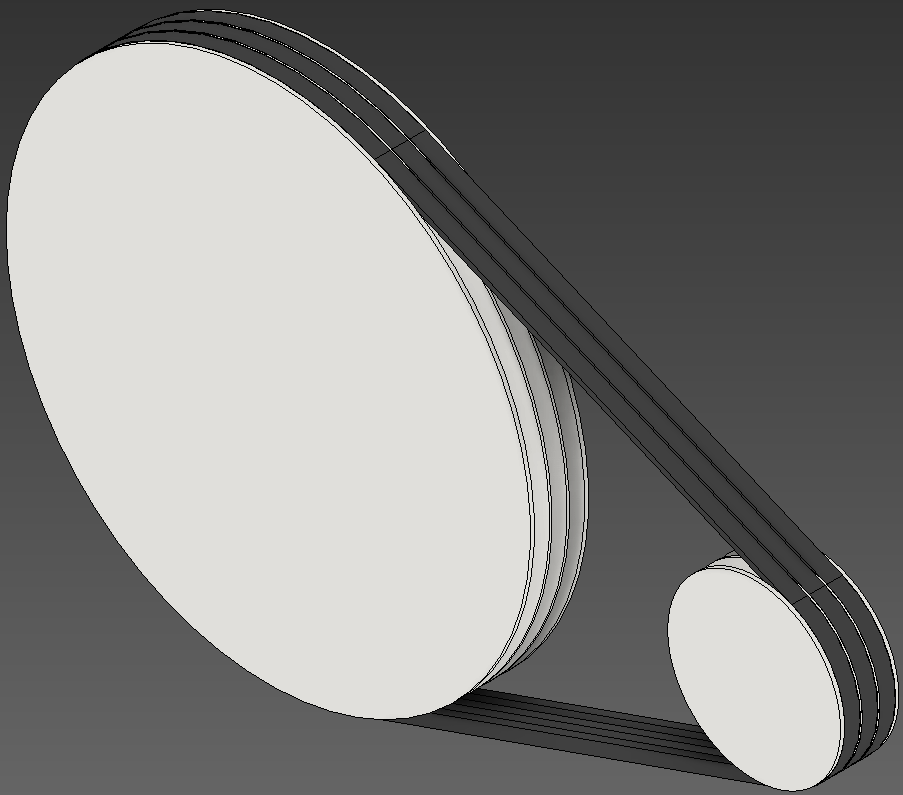
\includegraphics[width=150mm]{belt.png}
	\caption{Belt drive model}
	\label{belt}
\end{figure}

\subsubsection{The chain drive parameters table}
\begin{center}
	\rowcolors{2}{}{lightgray!20}
	\begin{longtable}{clr}
		\toprule
		No. & \multicolumn{1}{c}{Parameter} & \multicolumn{1}{c}{Result}\\
		\midrule\endfirsthead
		\toprule
		No. & \multicolumn{1}{c}{Parameter} & \multicolumn{1}{c}{Result}\\
		\midrule\endhead
		\bottomrule\endfoot
		\bottomrule
		\caption{Design specifications of the chain drive}
		\endlastfoot
		1 & Chain type & Roller Chain 16B-3-106\\
		2 & Number of chains & $ k=3 $\\
		3 & Number of chain links & $ X=106 $\\
		4 & Tangential force &$ F_p=2517.405\unit{(N)} $ \\
		5 & Tensile force on the tight side & $ F_1 =2540.238\unit{(N)}$\\
		6 & Tensile force on the slack side & $ F_2 = 22.834\unit{(N)} $\\
		7 & Radial force &$ F_r =2555.607\unit{(N)}$ \\
		8 & Contact angle & $ \alpha_1=132.11^\circ,\alpha_2=227.89^\circ $\\
		9 & Center distance &$ C= 626.966\unit{(mm)}$ \\
		10 & Drivsing sprocket diameter & $ D_{p} =170.421\unit{(mm)}$ \\
		11 & Driven sprocket diameter & $ D_{p} =679.304\unit{(mm)}$\\
	\end{longtable}
\end{center}
\begin{figure}
	\centering
	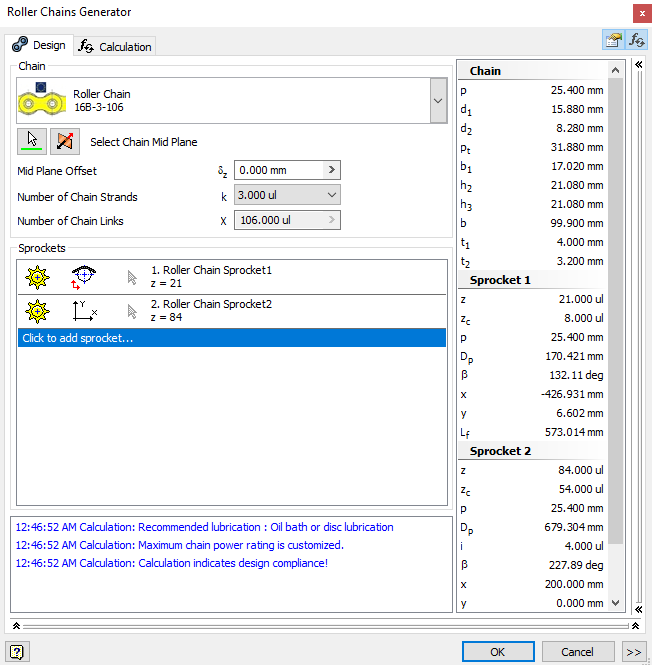
\includegraphics[width=150mm]{chaindesign.png}
	\caption{Chain design tab}
	\label{chaindesign}
\end{figure}
\begin{figure}
	\centering
	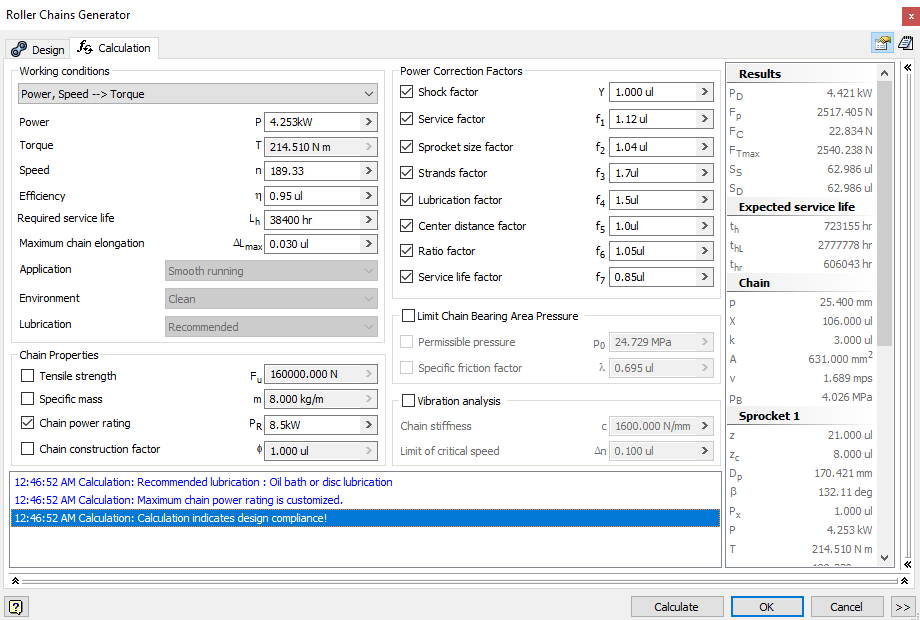
\includegraphics[width=150mm]{chaincalculation.png}
	\caption{Chain calculation tab}
	\label{chaincalculation}
\end{figure}
\begin{figure}
	\centering
	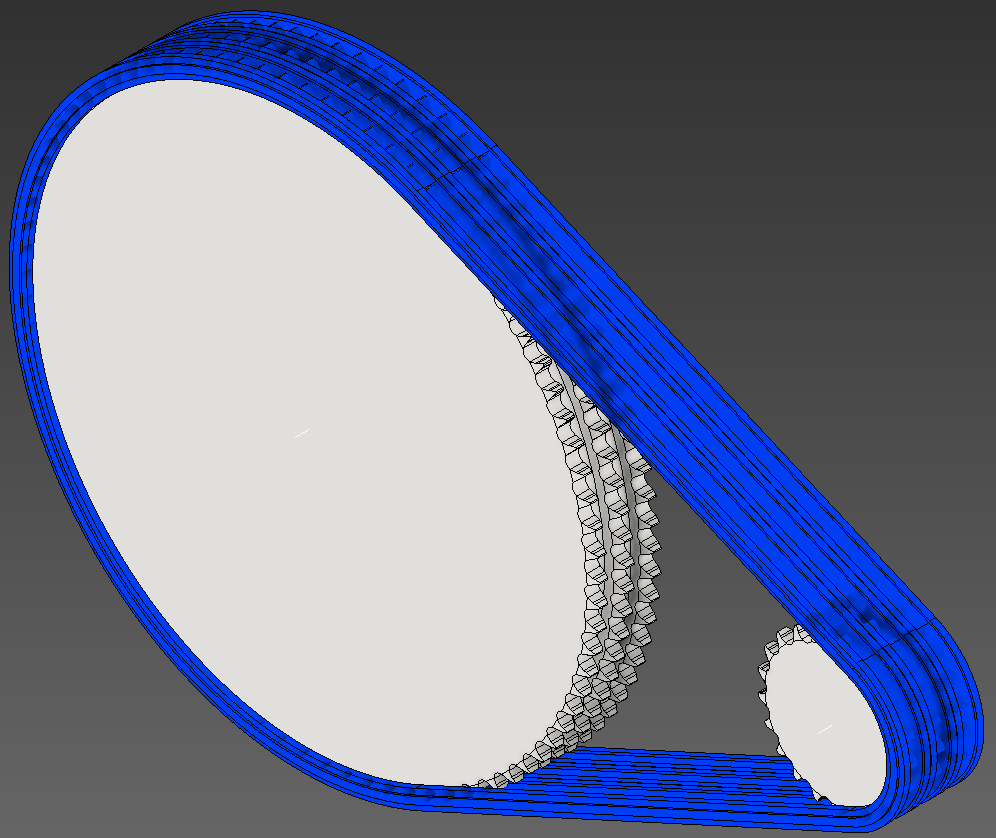
\includegraphics[width=150mm]{chain.png}
	\caption{Chain drive model}
	\label{chain}
\end{figure}

\section{Discussion and conclusions}
Students compare the computational results in Inventor software with the theoretical results. Then draw conclusions when we use Inventor software.\\
Calculation results from Autodesk Inventor are mostly similar to theoretical calculation. The software is a convenient tool for calculating and designing machine parts, which also provides a complete machine detail modules. The users can easily input and adjust the parameters and use the built-in libraries from the software.